\claude{
\section{Forecast selection and sampled-query estimation}\label{app:forecast_utility}
\paragraph{Training and observable.}
This experiment uses new 256-unit networks with the FORCE/RLS dynamics described in Appendix~\ref{app:controlled}. The seven task families are T1--T4, H2, H4, and M4. Each network trains for 40,000 updates with recurrent gain 1.2, integration step 0.1 and RLS updates every two steps; RLS starts at the identity. Target frequencies and random phases follow the generator construction above. An eighth, untrained reference has gain 1.5; it is not assumed to be chaotic and can settle to a fixed point. At frozen weights, each run has 5,000 burn-in steps and 8,192 recorded samples. The scalar is $\tanh(h_{t,2})$, using zero-based neuron index two. We use observations 4,096--6,143 as the prefix and 6,144--6,175 as the future target. No future values enter normalization, feature extraction, candidate fitting, or selection.

All trained networks are included, even when they fail to reproduce the higher-phase targets. Forecast errors measure their actual activity; the intended phase dimension is not assumed to have been learned.

\paragraph{Eight candidate forecasts.}
The pool comprises the last value, prefix mean, repetition at lag 314, ridge regression with 8 or 48 lags, five-nearest-neighbor regression with 8 or 48 lags, and ridge regression on 64 random Fourier features of a 48-lag input. Forecasts are direct 32-output regressions, fitted on all complete input/target pairs inside the prefix. Ridge uses penalty one and intercept penalty $10^{-8}$ on standardized inputs. The Fourier feature map has bandwidth $1/48$ and random seed 42. Nearest neighbors have uniform weights. Learned predictions are clipped at $\pm10$ prefix standard deviations. NMSE is squared forecast error averaged over the 32 future values and divided by prefix variance; no square root is taken. Prefix standard deviation below $10^{-10}$ triggers a shared persistence fallback, scored with variance floor $10^{-12}$ for every selector.

\paragraph{Selector training and search history.}
Each selector predicts the eight candidate losses and picks their minimum. Training uses seeds 601--618 (144 task records); three-fold cross-validation groups by seed. Four candidate selector architectures are considered equally for every feature set: decision trees of depth 2/3 with minimum leaf size eight, and 100-tree random forests of depth 3/6 with minimum leaf size five. Random seed is 42. Missing-value imputation and indicators are fit inside the training folds. The depth-two MG selector generally chooses nearest-neighbor prediction for cyclic records and ridge regression for more complex records. The task label and target phase dimension are never selector inputs.

An exploratory search over generators, neurons, horizons and sensor datasets preceded selection of the primary observable and forecast horizon. Seeds 619--630 identified the short-horizon candidate; seeds 631--650 tested it, after which stronger geometric competitors were added. All full-MG and geometric selector rules were then frozen before seeds 651--680 (30 new groups, 240 records). The sampled-query variant was proposed after measuring the cost of full MG and tested with the same frozen selectors on seeds 681--700 (20 further groups, 160 records). We report the two sets of test seeds separately. Resampling groups the eight tasks sharing each seed. The results concern this network family and task mixture; the bundled records document the search history.

\paragraph{Competitors and information access.}
All feature-based competitors use the same development runs and selector search. Cheap features are spectral entropy, normalized squared increments, lag-one correlation, minimum scalar recurrence error over lags 6--288, spectral peak concentration, linear trend, standard deviation, and mean. The geometric audit includes TwoNN and original Levina--Bickel pooling on the same delay cloud, its covariance participation ratio, permutation entropy of order five, and sample entropy with template length two and tolerance 0.2 standard deviations in Chebyshev distance. Held-out model search fits all eight candidates on four rolling prefixes with 32-point validation targets covering the last 128 known observations, then refits the chosen candidate on the entire prefix. Learned selectors receiving these validation errors have additional input and fitting cost. ``All except MG'' combines the cheap features, validation errors, and non-MG geometric features; ``all including MG'' adds MG to that same set. The oracle uses future errors and is only a lower bound. Table~\ref{tab:forecast_all} includes these stronger alternatives.

\begin{table}[ht]
\centering\small
\caption{\claude{Mean NMSE for all forecast selectors. Columns use distinct sets of test seeds; lower is better. Earlier MG was fit during the initial generator screen. The second set supports the query-budget comparison.}}
\label{tab:forecast_all}
\begin{tabular}{lrr}
\toprule
Selector & 30 seeds & 20 new seeds \\
\midrule
MG & 0.03138 & 0.03637 \\
Earlier MG rule & 0.03219 & --- \\
Best fixed on development runs & 0.04475 & 0.06041 \\
Held-out model search & 0.03224 & 0.04074 \\
Cheap features & 0.04517 & 0.05923 \\
Cheap + held-out search & 0.03617 & 0.03379 \\
Held-out errors & 0.03997 & 0.03424 \\
Held-out errors + MG & 0.03423 & 0.03167 \\
Cheap + MG & 0.03138 & 0.03637 \\
Cheap + held-out search + MG & 0.03534 & 0.03994 \\
TwoNN & 0.03540 & 0.04364 \\
Levina--Bickel & 0.04054 & 0.04732 \\
Delay covariance PR & 0.04397 & 0.06098 \\
Permutation entropy & 0.04484 & 0.05384 \\
Sample entropy & 0.04718 & 0.05954 \\
All features except MG & 0.03669 & 0.03939 \\
All features including MG & 0.03420 & 0.04071 \\
Oracle (future targets) & 0.00759 & 0.00847 \\
\bottomrule
\end{tabular}

\end{table}

On seeds 651--680, MG gives NMSE 0.03138 versus 0.03224 for ordinary held-out search; seed-bootstrap uncertainty includes no difference. On seeds 681--700, MG gives 0.03637 versus 0.04074: a 10.7\% lower sample mean, but the paired improvement interval is $[-0.00729,0.01758]$ over 20 seed groups (20,000 bootstrap resamples, random seed 811). MG wins on nine of those 20 groups. Cheap features plus learned held-out-error selection achieve 0.03379 and held-out-error features plus MG achieve 0.03167. Restricting seeds 651--680 to trained networks gives MG 0.03542 versus 0.03943 for TwoNN. The uncertainty against the strongest selectors remains.

\begin{figure*}[t]
\centering
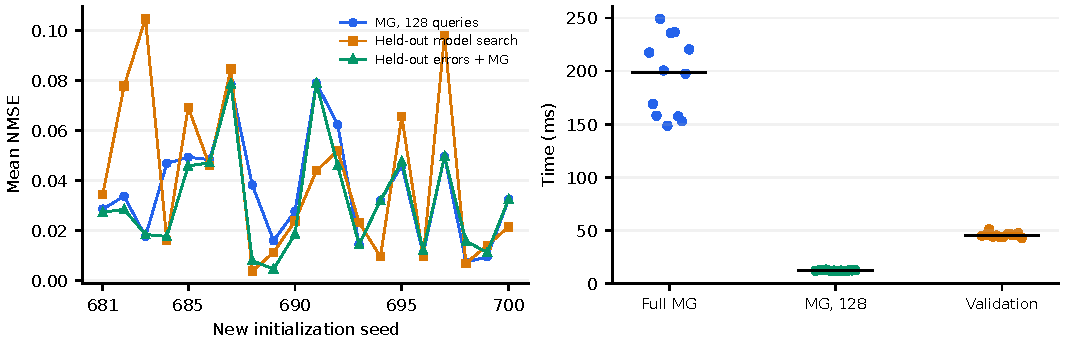
\includegraphics[width=.98\textwidth]{figures/forecast_utility.pdf}
\caption{\claude{Forecast selection: quality and cost. Left: each new seed group averaged over eight tasks; lower NMSE is better. Right: medians over seven timing repetitions for each of 12 matched inputs; black bars are medians over inputs.}}
\label{fig:forecast_utility}
\end{figure*}

\paragraph{Sampled-query MG.}
Use $E=20$, $k=20$, the adaptive lag of Appendix~\ref{app:settings}, an autocorrelation Theiler rule capped at 150, and dither seed 123. Standardization, floors, and temporal exclusion match the original kernel. For $n$ delay vectors, select $q=\min(128,n)$ distinct query indices uniformly across the record, with zero-based indices $\lfloor j(n-1)/(q-1)\rfloor$. All $n$ vectors remain candidate neighbors. With original time indices retained in the exclusion, compute
\begin{equation}
\widehat d_{\rm MG}^{(q)}=
\frac{q(k-1)-1}{\displaystyle\sum_{i\in Q}\sum_{j=1}^{k-1}\log(r_{ik}/r_{ij})}.
\label{eq:querymg}
\end{equation}
The approximation equals full MG when $Q$ contains every query. Numerical-floor checks use the queried distances and sums. Insufficient neighbors, nonfinite values or constant records yield unavailable estimates. The unchanged selector uses imputed scores to choose a forecast.

Distance computation uses blocks of 64 queries, followed by temporal exclusion, selection of $k$ admissible neighbors and pooling of log ratios. Its cost is $O(qnE)$ with bounded block memory. Both versions use the full neighbor cloud; comparison with the original KDTree therefore measures both query reduction and implementation changes.

On all 160 records from seeds 681--700, $q=128$ retains exactly the full-MG model choice and therefore the same forecast error. It does not produce an identical numerical estimate in general. The sensitivity budgets $q=64$ and $256$ also preserve those choices on these runs; $128$ is the primary budget, not a test-selected optimum. Twelve audited records check exact full-query agreement, tree/block neighbor-distance agreement, and affine rescaling; constant and nonfinite inputs are rejected. Forecast-choice agreement alone does not certify absolute active dimension.

\paragraph{Paired runtime procedure.}
Serial measurements use an Intel Core i5-12500H CPU, one numerical thread, seeds 681, 690, and 700 crossed with tasks T1, T2, H4, and T4, seven interleaved repetitions per input after warm-up. Medians per input are formed before aggregating the 12 inputs. Overall median times are 199.1 ms for full MG selection, 12.2 ms for $q=128$, and 45.3 ms for held-out model search. Median paired speed ratios are 16.3 and 3.7, respectively. Each includes the feature, selector, and final forecast fit. The held-out search performs 32 validation fits and one final fit; MG fits only its selected candidate. Disk access, acquisition of the common prefix, generation of the development bank, and offline selector training are excluded. These timings concern repeated selection from available records; elementary scalar statistics can be faster.

\section{Comparing intervention rules}\label{app:intervention_utility}
We compare MG with scalar baselines and fixed schedules for choosing when to stop training, freeze layers or prune units. All rules use the same development runs and candidate intervention times.

MNIST images are average-pooled to $14\times14$. A fixed balanced split uses 2,000 training images, 500 disjoint clean held-out evaluation images from the original training pool, and 2,000 official test images (split seed 1006). The network is a 196--128--128--10 ReLU MLP trained by Adam at $10^{-3}$, batch 64, for 2,048 updates. For stopping experiments, exactly 40\% or 60\% of training labels are replaced by a randomly selected wrong class. Each initialization seed has its own corruption mask. Observers are parameter norm and loss on a fixed random subset of 128 training examples with their possibly corrupted labels, not clean probe labels. The reported experiment replaces the earlier single-class probe pilot.

Candidates act at updates 256, 512, 768, 1,024, or 1,536; no threshold crossing means continuation to 2,048. Trailing windows have 256 samples, $E=10$, $\tau=1$, $k=10$, and $T=19$. MG competes with mean level, normalized trend, detrended standard deviation, increments, entropy, and lag-one correlation. All select one of the two observers and threshold direction/level with the same pilot search. Thresholds maximize pilot clean-validation accuracy minus $0.02$ times the arithmetic budget. We choose rules on seeds 0--2 and evaluate them on seeds 10--17. The evaluation trajectories predate the saved rule file, but rule fitting reads only pilot records; this was not prospective preregistration. A separate clean-validation checkpoint choice is an offline comparator, not a causal oracle for test accuracy. The no-intervention fallback uses the final recorded accuracy.

On clean training, freezing disables gradients through both hidden layers and continues fitting the final head. Pruning physically reduces both hidden layers to width 64, retaining units according to incoming-row norm times outgoing-column norm, copying retained weights/biases and sliced Adam moments. Each selected action time is executed from its saved checkpoint with the same minibatch RNG, then trained to update 2,048. Post-action outcomes are actual continuations, not inferred from the unchanged base path.

\begin{table*}[ht]
\centering\small
\caption{\claude{Eight-seed intervention results, including strong simple comparisons. MAC ratio is an approximate matrix-arithmetic budget relative to uninterrupted dense training; it excludes logging, monitoring, nonlinearities, optimizer work, and memory overhead and is not a wall-time speedup.}}
\label{tab:intervention_utility}
\begin{tabular}{lrrr}
\toprule
Task & Rule & Accuracy (\%) & MAC ratio \\
\midrule
Stop, 40\% noise & MG & 84.75 & 0.219 \\
Stop, 40\% noise & fixed & 84.72 & 0.250 \\
Stop, 40\% noise & level & 84.90 & 0.188 \\
Stop, 40\% noise & entropy & 84.67 & 0.203 \\
Stop, 40\% noise & never & 64.11 & 1.000 \\
Stop, 60\% noise & MG & 76.58 & 0.125 \\
Stop, 60\% noise & fixed & 76.58 & 0.125 \\
Stop, 60\% noise & level & 76.58 & 0.125 \\
Stop, 60\% noise & entropy & 76.58 & 0.125 \\
Stop, 60\% noise & never & 43.83 & 1.000 \\
Freeze, clean & MG & 91.53 & 0.535 \\
Freeze, clean & fixed & 91.32 & 0.515 \\
Freeze, clean & level & 91.32 & 0.515 \\
Freeze, clean & entropy & 91.32 & 0.515 \\
Freeze, clean & never & 92.29 & 1.000 \\
Prune, clean & MG & 92.44 & 0.572 \\
Prune, clean & fixed & 92.52 & 0.628 \\
Prune, clean & level & 92.50 & 0.618 \\
Prune, clean & entropy & 92.38 & 0.553 \\
Prune, clean & never & 92.29 & 1.000 \\
\bottomrule
\end{tabular}

\end{table*}

At 40\% noisy labels, MG stopping yields 84.75\% test accuracy at 448 updates on average, versus 64.11\% at the full budget; the mean-level rule yields 84.90\% at 384 updates. At 60\%, MG and fixed early stopping choose update 256 and both yield 76.58\%, versus 43.83\% for the full budget. For clean-data pruning, MG yields 92.44\% accuracy at 57.2\% of the dense arithmetic budget, versus 92.29\% for uninterrupted dense training. Fixed-time pruning yields 92.52\% at 62.8\%, while entropy gives 92.38\% at 55.3\%. The interventions help, but simpler rules can match them. Rule selection uses clean labeled pilot data and depends on the noise setting. Application to later runs avoids those labels; logging and monitoring remain extra costs.
}
